% command to make sure colorboxes don't create whitespace between code lines
\fboxsep=.6pt

% default settings for listings
\lstset{style=python, basicstyle=\scriptsize\ttfamily,escapechar=!}

\begin{frame}
    \centering
    \begin{figure}[H]
        
\includegraphics[keepaspectratio, width=0.7\paperwidth, height=\paperheight]{Logos/FreeFlower.pdf}
    \end{figure}
    Informatik: Programmieren\\
    \emoji{abacus} Kapitel 03: \textbf{Werte bei der Ausführung mitgeben}
\end{frame}



\begin{frame}[fragile]{Vieleck mit Variablen als \textit{direkt gesetzt} \emoji{handshake}}
\begin{columns}
\begin{column}{.7\textwidth}
\begin{lstlisting}
import turtle as t

# Anzahl Ecken und Seitenlänge
ecken = 5
laenge = 100

for _ in range(ecken):
    t.forward(laenge)
    t.right(360/ecken)
\end{lstlisting}
$\rightarrow$ Einfach, direkt!
\end{column}
\begin{column}{.3\textwidth}
\begin{figure}
\centering
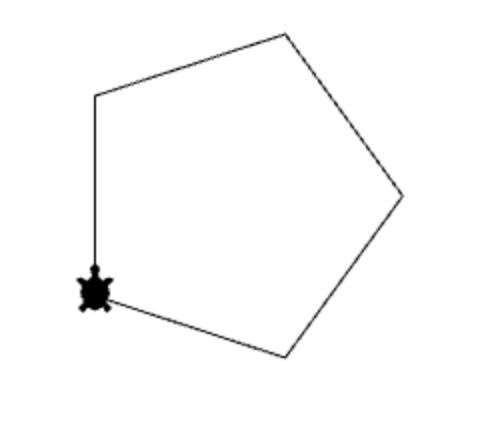
\includegraphics[width=\linewidth]{Grundlagen_Info/00_Programmieren/Figures/vieleck}
\end{figure}
\end{column}
\end{columns}
\end{frame}

\begin{frame}[fragile]{Vieleck mit \textit{hard-coded} Variablen \emoji{pencil}}
\begin{columns}
\begin{column}{.7\textwidth}
\begin{lstlisting}
import turtle as t

# Anzahl Ecken und Seitenlänge 
# sind direkt im Code
ecken = 5
laenge = 100

for _ in range(ecken):
    t.forward(laenge)
    t.right(360/ecken)
\end{lstlisting}
$\rightarrow$ Variablen sind fest!
\end{column}
\begin{column}{.3\textwidth}
\begin{figure}
\centering
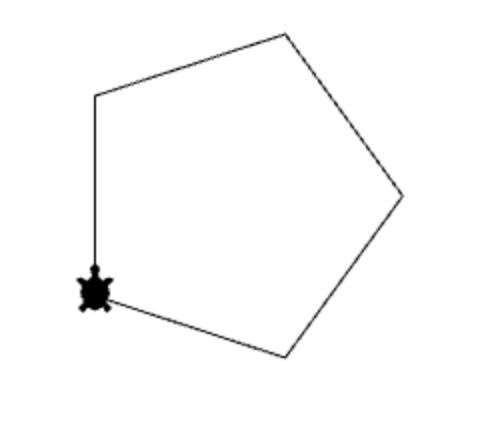
\includegraphics[width=\linewidth]{Grundlagen_Info/00_Programmieren/Figures/vieleck}
\end{figure}
\end{column}
\end{columns}
\end{frame}


\begin{frame}[fragile]{Vieleck mit Variablen, \textit{on-the-fly} \emoji{airplane}}
\begin{columns}
\begin{column}{.7\textwidth}
\begin{lstlisting}
import turtle as t

# Anzahl Ecken und Seitenlänge 
# mit input('...')
ecken = input("Wie viele Ecken?")
laenge = input("Seitenlänge?")

for _ in range(ecken):
    t.forward(laenge)
    t.right(360/ecken)
\end{lstlisting}
\end{column}
\begin{column}{.3\textwidth}
\begin{figure}
\centering
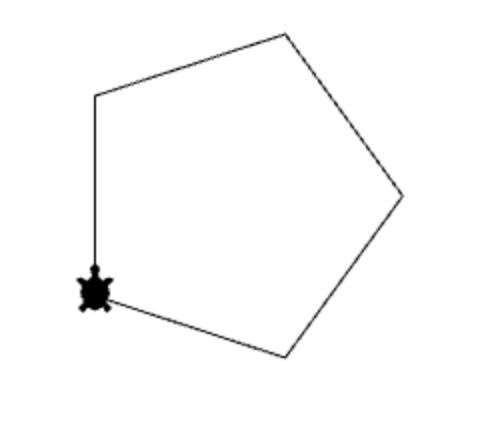
\includegraphics[width=\linewidth]{Grundlagen_Info/00_Programmieren/Figures/vieleck}
\end{figure}
\end{column}
\end{columns}
\end{frame}

\begin{frame}[fragile]{Vieleck mit Variablen, \textit{on-the-fly} \emoji{airplane}}{Mehrere Vielecke}
\begin{lstlisting}
import turtle as t

# Drei Vielecke wiederholt mit input
for wiederholung in range(3):
    ecken = input("Wie viele Ecken?")
    laenge = input("Seitenlänge?")
    for _ in range(ecken):
        t.forward(laenge)
        t.right(360/ecken)
\end{lstlisting}
$\rightarrow$ Demo
\end{frame}

\begin{frame}[fragile]{Zusammenfassung}
\begin{itemize}
\item Bei \lstinline|input| sind die Variablen-Werte vor der Programm-Ausführung \textit{unbekannt}!
\item Ermöglicht es, flexibel Variablenwerte \textit{während} der Programm-Ausführung zu definieren (\textit{on-the-fly} \emoji{airplane})
\end{itemize}
\end{frame}

\begin{frame}[fragile]{Auftrag}
\begin{itemize}
\item \abgabebox{Aufgaben 3.16}
\end{itemize}
\end{frame}